\documentclass[conference]{IEEEtran}
\IEEEoverridecommandlockouts


\usepackage{cite}
\usepackage{amsmath,amssymb,amsfonts}
\usepackage{graphicx}
\usepackage{textcomp}
\usepackage{xcolor}
\usepackage{booktabs}
\usepackage{multirow}
\usepackage{array}
\usepackage{url}
\usepackage{tikz}
\usepackage{pgfplots}
\pgfplotsset{compat=1.16}
\usetikzlibrary{shapes.geometric,arrows.meta}


\graphicspath{{figures/}}


% Uses the PNG if it exists in figures/, otherwise draws a labelled placeholder box
\newcommand{\figorbox}[3]{%
  \IfFileExists{figures/#1}%
    {\includegraphics[width=#2]{#1}}%
    {\fbox{\parbox[c][3.4cm][c]{\dimexpr#2-2\fboxsep-2\fboxrule\relax}{\centering\footnotesize TODO: #3\\(\texttt{figures/\detokenize{#1}})}}}}


\def\BibTeX{{\rm B\kern-.05em{\sc i\kern-.025em b}\kern-.08em
    T\kern-.1667em\lower.7ex\hbox{E}\kern-.125emX}}


\begin{document}


\title{When Is Reuse Safe? Regime-Aware Policy Transfer for Recurring Drift in Network Telemetry}


\author{
\IEEEauthorblockN{Neha Manoj}
\IEEEauthorblockA{
Ericsson Research\\
Bangalore,India\\
neha.manoj@ericsson.com
}
}


\maketitle


\begin{abstract}
Network telemetry drifts, and the standard fix, retraining, pays the full cost of
rebuilding the model every time. But network regimes recur: a congestion profile, a
radio configuration or an operator comes back. We ask whether a policy learned for a
regime can be reused when that regime returns, and when doing so is safe. Regime-Aware
Policy Transfer (RAPT) stores one ensemble policy per regime, retrieves it on
recurrence, and refits it when rolling accuracy shows it no longer fits. On four
network streams under a strict prequential protocol, RAPT uses 48--92\% less adaptation
CPU than full retraining. Macro-F1 is lower on all four streams, significantly so on
two. The clearest failure is UGR'16, where regime identifiers recur but the
feature-to-label mapping does not. Blind reuse drops macro-F1 to $0.836$, and a parity
refit that checks the reused policy's recent accuracy recovers it to $0.928$. So reuse
keyed on regime identity alone is unsafe, and reuse with a performance check is not. On
5G Campus, a cost-aware refit configuration matches full retraining within measurement
noise ($\Delta$macro-F1 $=+0.0022$, $p=0.31$) at about 40\% less adaptation CPU. Two
other mechanisms failed under measurement and we report them: a relative-degradation
trigger that cannot fire on a policy that was poor from the start, and an incremental
learner that was worse on both accuracy and cost.
\end{abstract}


\begin{IEEEkeywords}
concept drift, network telemetry, online learning, adaptive ensembles,
regime-aware learning, computationally efficient adaptation
\end{IEEEkeywords}


\section{Introduction}


The data seen by network monitoring systems does not stay the same for long. Load,
radio conditions, subscriber mobility and configuration changes each move the
distribution, and a classifier fitted on a period of a 5G testbed or an ISP netflow
archive will not stay accurate for very long. Retraining once performance drops is the
standard answer. It works, but it has to be paid for again every time, and with
high-rate telemetry the total spent on rebuilding models may end up above what it costs
to serve predictions. Lightweight detection and adaptation frameworks for constrained devices already exist
\cite{9427288}, and many good detectors decide \emph{when} to adapt
\cite{bifet2007learning,page1954continuous,gama2004learning,baena2006early,ross2012exponentially,dos2016fast,brockhoff2020time},
but they make no use of how the change is structured. Conditions in networks often come
back. A weekday congestion profile, a radio configuration or an operator-specific QoS
regime may go away and return later. Some of the earliest work in the field was driven
by recurring concepts \cite{schlimmer1986incremental,widmer1994combining}, and still
the usual practice is to learn again from scratch, even though the model being thrown
away may well be the right one.


The question we ask here is whether the discarded information can be kept and used. RAPT
keeps a repository of adaptation policies, each indexed by an operating regime. At a
regime boundary it looks up whether the incoming regime already has a stored policy.
When it does, that ensemble is retrieved at close to zero adaptation cost, and when it
does not, a new policy is trained and added to the repository. Since a retrieved policy
can be wrong if the label relationship in that regime has changed, RAPT also follows
its streaming accuracy and refreshes the policy if needed. 


 If regimes recur with stable label
semantics, reuse keeps accuracy and removes most of the adaptation cost. If regimes
recur but the feature-to-label relationship has moved, reuse brings back a stale policy
and accuracy suffers, and the repair mechanism is the reason the approach still works
in that setting. Our contributions are as follows:
\begin{itemize}
\item a regime-conditioned policy-transfer mechanism that stores and retrieves
ensemble policies by regime;
\item a monitoring and refresh strategy whose cost-aware configuration matches
full-retraining accuracy at a fraction of the cost;
\item an evaluation on four network streams under one prequential protocol,
against four established drift detectors;
\item a failure analysis covering harmful blind reuse, a trigger that cannot fire
by construction, and an incremental learner that loses on both axes.
\end{itemize}


\section{Related Work}


\subsection{Concept and Data Drift}
Drift in a data stream is usually sorted into two cases. Under covariate shift the
marginal $P(X)$ changes while $P(Y\mid X)$ holds, and under concept drift it is the
conditional $P(Y\mid X)$ that changes \cite{gama2004learning,lu2018learning}. Surveys
have catalogued the taxonomies and adaptation strategies built up over the years
\cite{khamassi2018discussion}. The story starts with STAGGER and its recurring concepts
\cite{schlimmer1986incremental}, and with Widmer's analysis of robustness against
flexibility \cite{widmer1994combining}. 


\subsection{Drift Detection}


ADWIN compares sub-window means inside an adaptive window \cite{bifet2007learning},
and Page-Hinkley is a sequential cumulative-sum procedure \cite{page1954continuous}.
DDM and EDD follow the error rate together with its variance
\cite{gama2004learning,baena2006early}. RDDM was designed to give fewer false alarms
\cite{barros2017rddm}, while the EDMA and EWMA charts track an exponentially weighted
moving average of the error \cite{ross2012exponentially}. A separate family needs no
labels and tests the features directly. Examples use Hoeffding bounds
\cite{frias2014online}, an incremental Kolmogorov--Smirnov statistic
\cite{dos2016fast}, or the earth-mover distance \cite{brockhoff2020time}, and
lightweight versions exist for constrained IoT deployments \cite{9427288}. 


\subsection{Adaptive and Online Learning}
Online ensembles handle drift by updating their members as new data arrives. Dynamic
weighted majority weights each learner by its recent accuracy and adds or drops
learners along the way \cite{JMLR:v8:kolter07a}; it grew out of earlier methods that
minimize disagreement on drifting concepts \cite{helmbold1994tracking}. Adaptive random
forests pair online bagging with drift-aware tree replacement
\cite{gomes2017adaptive}, and the accuracy-updated ensemble reweights its components
when drift appears \cite{brzezinski2013reacting}. Similar designs have been proposed
for social big-data and IoT streams \cite{abbasi2021elstream,yang2021pwpae}.
Single-pass incremental learners, of which Hoeffding trees are the standard example,
keep memory use and per-example update cost bounded \cite{domingos2000mining}. The
detectors and incremental learners in our experiments come from the River library
\cite{montiel2021river}. All of this work is about \emph{how} a model gets
updated. None of it considers fetching a model that is already good enough. In
Section~\ref{sec:ablation} we test one incremental learner against our approach, and
on our stream it does not improve the accuracy--cost trade-off.


\subsection{Transfer under Recurring Conditions}
Transfer learning moves representations or parameters learned on a source task over to
a related target task \cite{pan2010transfer}. The idea of holding on to learned structure
has a long history, with roots in work on the role of forgetting
\cite{markovitch1988role} and on the cost of reusing compiled knowledge chunks
\cite{tambe1988some}.
 It saves a fitted policy
with its regime identity and retrieves the two together. The decision it makes is
whether any adaptation is needed, and how to adapt is left aside. With no recurrence,
the mechanism collapses into ordinary retraining.


\section{Problem Formulation}


We treat the data as a chronological stream $x_1, x_2, \dots$, where
$x_t \in \mathbb{R}^d$ is a feature vector and $y_t \in \{1,\dots,C\}$ is its label. The
label is unknown until the prediction for $x_t$ has been issued. The stream is divided
into fixed-size windows $W_1, \dots, W_T$, and each window $W_k$ is tagged with a regime
identifier $r_k \in \mathcal{R}$. A regime is a semantically defined operating
condition, such as a network scenario or a time-of-day block. It is not a cluster label.
A \emph{policy} $\pi$ is a fitted model plus its decision rule, and the repository is a
mapping $\mathcal{P}: \mathcal{R} \rightarrow \pi$ that is filled in as new regimes show
up. Whenever the stream moves from $r_{k-1}$ to $r_k$, the controller picks an action
$a_k \in \{\textsc{reuse}, \textsc{train}\}$. It reuses $\mathcal{P}(r_k)$ when that
exists, and trains a new policy on the recent buffer when it does not. Let $M(\pi, W)$
be a performance measure, which is macro-F1 in this paper, and let $c(\pi)$ be the cost
of producing $\pi$ in adaptation CPU time. The objective is to hold $M(\cdot, W_k)$ near
the level a freshly trained policy would reach while making $\sum_k c(a_k)$ as small as
possible.


Reuse rests on an assumption, namely that $P(Y \mid X, r_k)$ has not changed since the
policy was stored. If the regime identifier returns after the conditional relationship
has shifted, the stale policy gets applied and nothing flags it. The hard part is
separating a recurring regime from a recurring label relationship.


\section{Proposed Method: RAPT}
\label{sec:method}


\subsection{Architecture and Repository}
RAPT sits between the stream and the model and makes one decision at each regime
boundary. The active policy predicts each window, and the window is scored when its
labels arrive. A change of policy happens only at a regime transition or when
monitoring reports degradation.


% ---------- NEW FIGURE: method overview ----------
\begin{figure*}[!t]
\centering
\resizebox{\textwidth}{!}{%
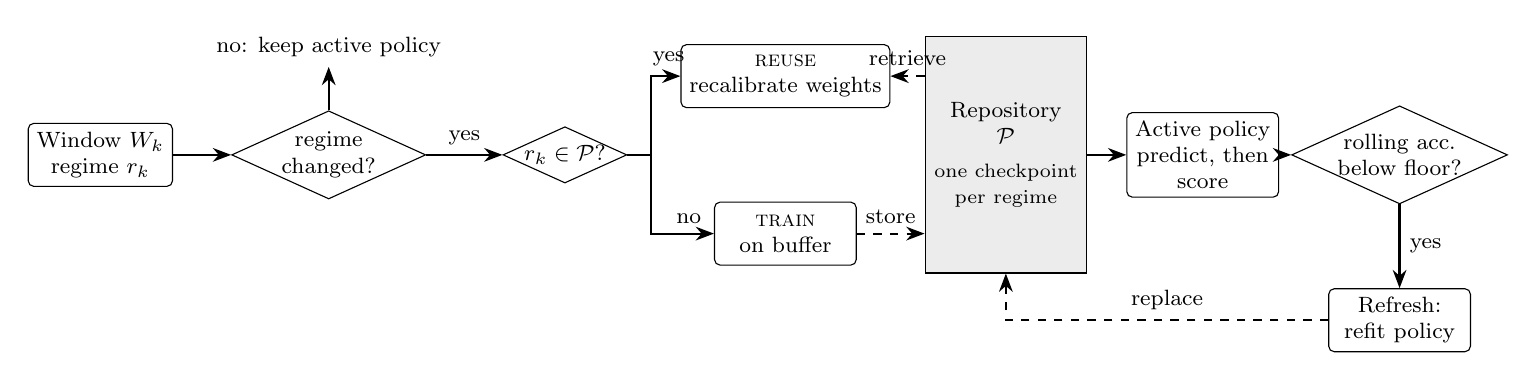
\begin{tikzpicture}[>=Stealth, font=\footnotesize,
  box/.style={draw, rounded corners=2pt, align=center, minimum height=8mm, minimum width=18mm, inner sep=3pt},
  dec/.style={draw, diamond, aspect=2.2, align=center, inner sep=0pt},
  repo/.style={draw, align=center, fill=gray!15, minimum height=30mm, minimum width=19mm},
  flow/.style={->, thick},
  mem/.style={->, dashed, thick}]
\node[box]  (win)  at (0,0)     {Window $W_k$\\regime $r_k$};
\node[dec]  (chg)  at (2.9,0)   {regime\\changed?};
\node[dec]  (hit)  at (5.9,0)   {$r_k \in \mathcal{P}$?};
\node[box]  (reuse) at (8.7,1.0) {\textsc{reuse}\\recalibrate weights};
\node[box]  (train) at (8.7,-1.0){\textsc{train}\\on buffer};
\node[repo] (repo) at (11.5,0)  {Repository\\$\mathcal{P}$\\[1mm]\scriptsize one checkpoint\\\scriptsize per regime};
\node[box]  (act)  at (14.0,0)  {Active policy\\predict, then\\score};
\node[dec]  (mon)  at (16.5,0)  {rolling acc.\\below floor?};
\node[box]  (ref)  at (16.5,-2.1){Refresh:\\refit policy};


\draw[flow] (win) -- (chg);
\draw[flow] (chg) -- node[above]{yes} (hit);
\draw[flow] (chg.north) -- ++(0,0.55) node[above]{no: keep active policy} ;
\draw[flow] (hit.east) -- ++(0.3,0) |- node[pos=0.8,above]{yes} (reuse.west);
\draw[flow] (hit.east) -- ++(0.3,0) |- node[pos=0.8,above]{no} (train.west);
\draw[mem] (repo.west |- reuse.east) -- node[above]{retrieve} (reuse.east);
\draw[mem] (train.east) -- node[above]{store} (repo.west |- train.east);
\draw[flow] (repo.east) -- (act.west);
\draw[flow] (act.east) -- (mon.west);
\draw[flow] (mon.south) -- node[right]{yes} (ref.north);
\draw[mem] (ref.west) -| node[pos=0.25,above]{replace} (repo.south);
\end{tikzpicture}}
\caption{RAPT overview. At each regime boundary the controller looks up the incoming
regime in the repository and either reuses the stored policy or trains and stores a new
one. The active policy predicts and is scored as labels arrive. A monitor refits the
policy and replaces its checkpoint when rolling accuracy degrades. Solid arrows are
control flow, dashed arrows are repository reads and writes.}
\label{fig:overview}
\end{figure*}
% ---------- END NEW FIGURE ----------


We represent a regime with its semantic identifier and do not learn a clustering.  What we give up is that
the mechanism requires a usable regime signal; see Section~\ref{sec:limitations}. The
repository holds one checkpoint per regime, made up of the fitted ensemble, its
soft-voting weights, and timestamps for creation and last access. Checkpoints are
immutable.


\subsection{Matching and Transfer}
Matching uses the regime identifier. On a transition to regime $r$, the controller tests
whether $r \in \mathcal{P}$. The enhanced variant also applies a fingerprint-similarity
gate, which requires the feature summary of the current window to be close to the
fingerprint saved when the checkpoint was created. The effect is to relax the question
``has this regime been seen?'' into ``has a sufficiently similar instance been seen?''.


When reuse goes ahead, the retrieved ensemble becomes the active policy, and its
soft-voting weights can be recalibrated using the most recent buffered window.
Calibration computes the recent accuracy of the two components and renormalizes their
weights. It covers at most the last 50 observations and is skipped when fewer than 20
are available, so its cost is small and fixed. If no checkpoint exists, we train a new
policy from a class-anchored buffer and store it. The buffer holds a stratified slice of
the training prefix. All adaptive models here use it in the same way, which stops a
refit from collapsing onto a single class when the recent window has only one.


\subsection{Monitoring, Refresh, and Fallback}
We use two monitoring rules, and how they differ is one of our findings. The
\emph{absolute} rule triggers when rolling accuracy goes under a fixed floor. The
\emph{relative} rule triggers when accuracy has dropped by more than a fixed margin from
a decayed reference, which is built from that policy's own earlier accuracy.
 A relative rule cannot catch a
policy that was never good, because the reference decays toward the poor level and so
the gap it looks for never appears.


A refresh rebuilds the active policy from the recent buffer and replaces its checkpoint,
and any later reuse then gets the refreshed policy. In the default refresh, the
100-tree ensemble is refit on a 1000-observation buffer. The cost-aware refresh has the
same trigger but refits 20 trees on a 300-observation buffer.RAPT-Enhanced contains two additions. \emph{Buffer-blended novelty refitting} refits a
novel regime on a 1500-observation buffer, where the original used 500.
\emph{Selective parity refitting} refits a reused policy and replaces its checkpoint
whenever rolling accuracy falls under a parity threshold over a short window. This
targets stale reuse directly.  When there is no checkpoint, or the similarity gate
turns down the one that exists, the controller trains a fresh policy and stores it under
the incoming regime identifier. 
\section{Experimental Methodology}\label{sec:protocol} 
\subsection{Datasets} 
Four datasets are summarized in Tab.~\ref{tab:datasets}; all are real network traces.
\emph{5G Campus} is a testbed QoS stream with delay metrics labelled GOOD, DEGRADED or
BAD from the 90th-percentile delay of the next window; each of the three scenarios recurs
fourteen times. \emph{UGR'16} is aggregated ISP netflow with 134 features. Because the
calibration split contains almost no labelled attack traffic, we use the first thirty days
of labelled data, one sample per minute (43{,}200 samples); time-of-day crossed with
weekday/weekend gives twelve regimes and 168 recurrences. \emph{NordicDat} is a
cross-border LTE/5G predictive-QoS trace \cite{nordicdat} whose regimes are operators.
Both of these label the median delay of the next window into three classes. \emph{5G NR}
is a simulated end-to-end latency stream \cite{nrlatency} of 499 windows of 500 packets
across four regimes (ABCDACBDAB), labelled with the same rule as Campus.


\begin{table}[hbt!] 
\small 
\caption{Datasets used in evaluations. Recurrences denote occurrences where a particular regime is revisited.} 
\label{tab:datasets} 
\centering 
\begin{tabular}{@{}llrrrr@{}}
\toprule
\textbf{Property} & \textbf{Campus} & \textbf{UGR'16} & \textbf{Nordic} & \textbf{5G NR}\\
\midrule
Samples & 1,799 & 43,200 & 91,455 & 249,500\\
Features & 19 & 134 & 16 & 12\\
Classes & 3 & 2 & 3 & 3\\
Windows & 179 & 180 & 182 & 499\\
Window size & 10 & 240 & 500 & 500\\
Regimes & 3 & 12 & 3 & 4\\
Recurrences & 14 & 168 & 17 & 6\\
\bottomrule
\end{tabular} 
\end{table}


\subsection{Preprocessing, Ordering, and Leakage Control} 
All four streams undergo the exact same processing. First, all four streams undergo sorting by row according to timestamp. Then, all identifier and constant columns are dropped. Finally, only those features that are numeric are retained. Any infinite values present within a stream are treated as missing. Any rows that lack a target value are deleted. Any remaining gaps are then filled using medians computed solely from the training prefix. Target thresholds and any scale-related statistics also derive from that prefix. None of the streams are shuffled. The prefix is the first twenty percent of windows: thirty-six for the three cross-dataset streams and ninety-nine for 5G NR. That prefix is completely excluded from evaluation, and that is the sole source of target thresholds. The order of operations is predict → evaluate → adapt for every window prior to its labels being used for adaptation. Regime annotation occurs directly from reading the stream. Therefore, no derivation of annotation can occur based upon the target.


\subsection{Models And Detectors} 
Each of the five primary models utilizes exactly the same base architecture and the same retraining buffer. Therefore, any variation between them is due to their respective adaptation mechanisms only. The base is an ensemble of a random forest classifier and an extra-trees classifier, both having fifty trees of depth seven. Frozen is trained once on the prefix and receives no subsequent updates. Event-Driven will update when window accuracy falls below a fixed threshold. Full Retraining will recreate/rebuild the model at every regime transition. RAPT and RAPT-Enhanced represent the controller(s) explained in Section~\ref{sec:method}.


ADWIN, Page-Hinkley, EDD and EDMA operate within the same retraining harness, with identical model, buffer, capacity and minimum-retrain-interval. They differ only by how they detect triggers. We pre-set their parameters in advance and did not adjust them via testing against our test streams (ADWIN $\delta$ = .002; Page-Hinkley min = Thirty; THRESHOLD = Fifty; EDD WARNING = Two; DRIFT = Three; EDMA $\alpha$ = .2 k = Two). Since none of our streams include true ground truth drift boundary indicators we report detected events, adaptation costs and predictive performance. Precision and Recall were not reported for our detectors.


\subsection{Metrics And Statistics} 
Performance is evaluated through macro-F1, Accuracy, Precision and Recall measures. Costs may be measured in two fashions. Adaptation CPU denotes CPU time exclusively devoted to adaptation routines while Runtime indicates Total Streaming Time. A reduction in Adaptation Time does not necessarily translate into a proportional reduction in Total Runtime.


Each experiment had seeds [42,43,44,45,46]. Therefore we report Mean and Standard Deviation for each measure. For comparison purposes we use the Wilcoxon Signed-Ranked Test for paired comparisons along with Cohen’s d. With respect to pairing by Window there would be approximately 143–146 observations. When paired by Seed we would have n = 5 with a minimum two-sided p-value available to us of .0625. If a result shows no significance we state that no difference was demonstrated between methods.


\subsection{Predictive Performance}
Table~\ref{tab:primary} holds the primary comparison, and Fig.~\ref{fig:primary} shows
the macro-F1 values side by side.


\begin{table*}[t]
\caption{Primary comparison and cost, mean over seeds 42--46. Bold marks the
best macro-F1 per stream; CPU and runtime in seconds, events are counts.}
\label{tab:primary}
\centering
\scriptsize
\begin{tabular}{@{}llcccccccc@{}}
\toprule
\textbf{Dataset} & \textbf{Model} & \textbf{F1} & \textbf{Acc.} & \textbf{Prec.} & \textbf{Rec.} & \textbf{CPU (s)} & \textbf{Run (s)} & \textbf{Retr.} & \textbf{Reuse} \\
\midrule
\multirow{5}{*}{5G Campus}
 & Frozen & $0.9364 \pm 0.0023$ & $0.9822 \pm 0.0006$ & $0.9379 \pm 0.0025$ & $0.9377 \pm 0.0017$ & 0.0000 & 1.2482 & 0 & -- \\
 & Event-Driven & $0.9636 \pm 0.0006$ & $0.9908 \pm 0.0003$ & $0.9637 \pm 0.0008$ & $0.9646 \pm 0.0002$ & 0.1080 & 1.3926 & 1 & -- \\
 & Full Retraining & $\mathbf{0.9836 \pm 0.0013}$ & $0.9951 \pm 0.0000$ & $0.9838 \pm 0.0015$ & $0.9843 \pm 0.0012$ & 1.4008 & 2.6677 & 14 & -- \\
 & RAPT & $0.9381 \pm 0.0016$ & $0.9838 \pm 0.0003$ & $0.9393 \pm 0.0017$ & $0.9392 \pm 0.0016$ & 0.2292 & 1.4931 & 2 & 12 \\
 & RAPT-Enhanced & $0.9381 \pm 0.0016$ & $0.9838 \pm 0.0003$ & $0.9393 \pm 0.0017$ & $0.9392 \pm 0.0016$ & 0.2337 & 2.1046 & 2 & 12 \\
\midrule
\multirow{5}{*}{UGR'16}
 & Frozen & $\mathbf{0.9690 \pm 0.0029}$ & $0.9899 \pm 0.0007$ & $0.9795 \pm 0.0030$ & $0.9662 \pm 0.0028$ & 0.0000 & 2.4914 & 0 & -- \\
 & Event-Driven & $0.8972 \pm 0.0277$ & $0.9898 \pm 0.0013$ & $0.9042 \pm 0.0269$ & $0.8955 \pm 0.0280$ & 0.5754 & 3.1303 & 3 & -- \\
 & Full Retraining & $0.9595 \pm 0.0012$ & $0.9873 \pm 0.0007$ & $0.9726 \pm 0.0014$ & $0.9580 \pm 0.0015$ & 23.6318 & 26.2627 & 144 & -- \\
 & RAPT & $0.8360 \pm 0.0262$ & $0.9635 \pm 0.0182$ & $0.8527 \pm 0.0205$ & $0.8336 \pm 0.0294$ & 1.9711 & 4.4990 & 11 & 133 \\
 & RAPT-Enhanced & $0.9276 \pm 0.0123$ & $0.9880 \pm 0.0017$ & $0.9375 \pm 0.0117$ & $0.9251 \pm 0.0123$ & 2.7182 & 5.9329 & 11 & 133 \\
\midrule
\multirow{5}{*}{NordicDat}
 & Frozen & $0.2779 \pm 0.0224$ & $0.4770 \pm 0.0123$ & $0.4215 \pm 0.0226$ & $0.2487 \pm 0.0229$ & 0.0000 & 2.5488 & 0 & -- \\
 & Event-Driven & $0.2547 \pm 0.0177$ & $0.4583 \pm 0.0367$ & $0.3909 \pm 0.0208$ & $0.2274 \pm 0.0151$ & 0.2533 & 2.8435 & 2.2 & -- \\
 & Full Retraining & $\mathbf{0.4227 \pm 0.0299}$ & $0.5694 \pm 0.0075$ & $0.4938 \pm 0.0233$ & $0.4085 \pm 0.0293$ & 2.2034 & 4.7593 & 18 & -- \\
 & RAPT & $0.3818 \pm 0.0184$ & $\mathbf{0.6172 \pm 0.0127}$ & $0.4703 \pm 0.0185$ & $0.3582 \pm 0.0192$ & 0.2594 & 2.8257 & 2 & 16 \\
 & RAPT-Enhanced & $0.3783 \pm 0.0321$ & $0.5677 \pm 0.0222$ & $0.4600 \pm 0.0307$ & $0.3614 \pm 0.0318$ & 2.6492 & 5.8812 & 2 & 16 \\
\midrule
\multirow{5}{*}{5G NR Lat.}
 & Frozen & $0.8961 \pm 0.0099$ & $0.9075 \pm 0.0061$ & $0.9314 \pm 0.0083$ & $0.8798 \pm 0.0085$ & 0.0000 & 1.7862 & 0 & -- \\
 & Event-Driven & $0.8903 \pm 0.0107$ & $0.9055 \pm 0.0060$ & $0.9475 \pm 0.0085$ & $0.8688 \pm 0.0083$ & 1.0406 & 2.7561 & 11 & -- \\
 & Full Retraining & $\mathbf{0.9027 \pm 0.0059}$ & $0.9145 \pm 0.0045$ & $0.9478 \pm 0.0053$ & $0.8829 \pm 0.0055$ & 0.7636 & 2.4689 & 9 & -- \\
 & RAPT & $0.8894 \pm 0.0110$ & $0.9025 \pm 0.0068$ & $0.9258 \pm 0.0103$ & $0.8737 \pm 0.0092$ & 0.3955 & 2.1112 & 3 & 6 \\
 & RAPT-Enhanced & $0.8915 \pm 0.0117$ & $0.9055 \pm 0.0076$ & $0.9348 \pm 0.0106$ & $0.8737 \pm 0.0098$ & 0.8609 & 2.5710 & 3 & 6 \\
\bottomrule
\end{tabular}
\end{table*}


On 5G Campus every model is close to saturation. Full Retraining has the best macro-F1
($0.9836 \pm 0.0013$), while RAPT and RAPT-Enhanced both land at $0.9381 \pm 0.0016$.
That is $0.0455$ lower, and the gap is significant ($p = 2.6 \times 10^{-4}$,
$d = -0.32$). 


UGR'16 is where the assumptions of the mechanism fail, and it teaches us the most. Frozen
has the highest macro-F1 ($0.9690 \pm 0.0029$), which is consistent with attacks being
sparse and clustered. RAPT reaches only $0.8360 \pm 0.0262$. This is $0.1236$ below Full
Retraining ($p = 2.6 \times 10^{-11}$, $d = -0.67$) and the worst of the five models,
despite its 133 reuses. The twelve regimes do recur, and their identifiers stay valid
throughout the 30-day block, but the mapping from netflow features to attack labels does
not stay put.  When RAPT-Enhanced parity-refits a reused
policy that has degraded, macro-F1 recovers to $0.9276 \pm 0.0123$. The gain of $0.0917$
($p = 5.4 \times 10^{-9}$, $d = 0.56$) is the one statistically supported improvement of
a variant over another on this stream.


NordicDat is hard to predict. Frozen scores $0.2779 \pm 0.0224$, adaptation helps, and
Full Retraining gets $0.4227 \pm 0.0299$ against $0.3818 \pm 0.0184$ for RAPT. The
deficit of $0.0409$ is not significant ($p = 0.255$, $d = -0.12$). RAPT does have the
highest accuracy on this stream ($0.6172 \pm 0.0127$ against $0.5694 \pm 0.0075$). On 5G NR the five models are only $0.0133$ apart. Taken together, the predictive results give no basis for saying that RAPT improves
accuracy. Full Retraining has the best macro-F1 on three of the four streams, and RAPT
sits below it on all four. The case for RAPT depends on cost, and on knowing when reuse
is safe.


\begin{figure}[t]
\centering
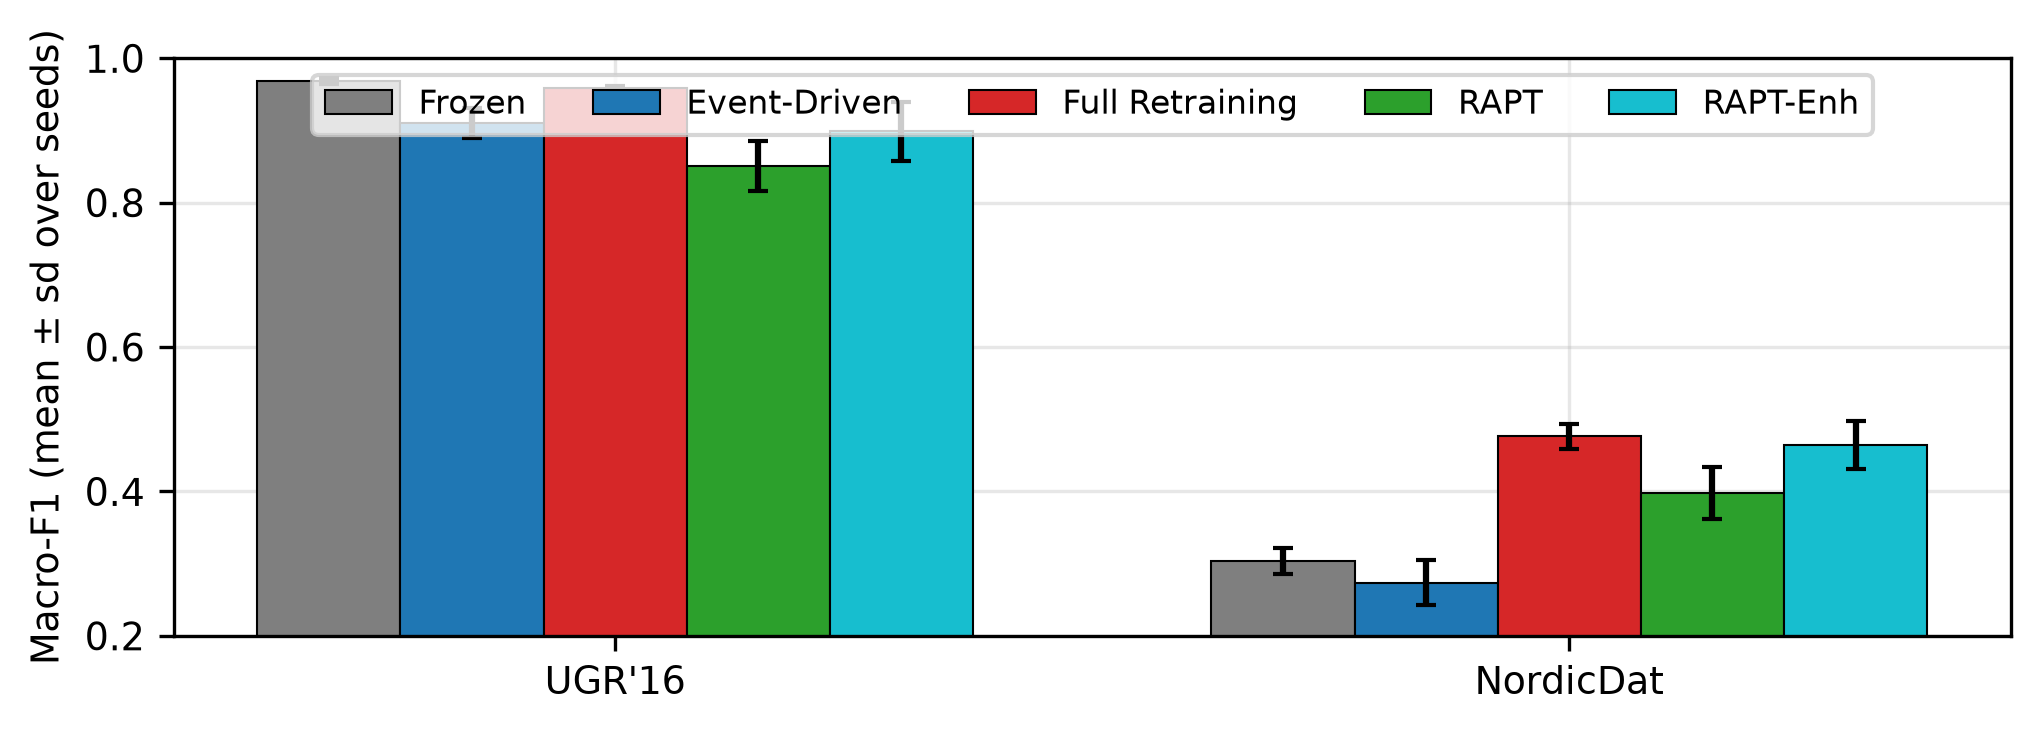
\includegraphics[width=\columnwidth]{primary_performance.png}
\caption{Macro-F1 on the two largest cross-dataset streams. On UGR'16, RAPT tracks
the frozen baseline and not the retrained models, which is the signature of stale
policy reuse. On the 5G NR stream all five models are within $0.0133$.}
\label{fig:primary}
\end{figure}


% ---------- NEW FIGURE: UGR'16 rolling accuracy ----------
\begin{figure}[t]
\centering
\figorbox{ugr_rolling_accuracy.png}{\columnwidth}{UGR'16 rolling accuracy over windows for RAPT, RAPT-Enhanced and Full Retraining}
\caption{Rolling accuracy over evaluation windows on UGR'16. RAPT sags once reused
policies go stale, and the parity refit in RAPT-Enhanced pulls accuracy back toward
Full Retraining. Vertical ticks mark novelty refits: the first window of each new
regime, where RAPT trains a fresh policy.}
\label{fig:ugr_rolling}
\end{figure}
% ---------- END NEW FIGURE ----------


\subsection{Computational Cost and Policy Reuse}
Table~\ref{tab:primary} also lists adaptation and total cost, and Fig.~\ref{fig:cost} compares adaptation CPU. Relative to Full Retraining, the cost falls on every stream:
from $1.4008$ to $0.2292$\,s on 5G Campus ($-83.6\%$), from $23.6318$ to $1.9711$\,s on
UGR'16 ($-91.7\%$), from $2.2034$ to $0.2594$\,s on NordicDat ($-88.2\%$), and from
$0.7636$ to $0.3955$\,s on 5G NR ($-48.2\%$). Full Retraining retrains at every regime
transition, meaning 14, 144, 18 and 9 times. RAPT retrains 2, 11, 2 and 3 times and
retrieves a stored policy 12, 133, 16 and 6 times.


\begin{figure}[t]
\centering
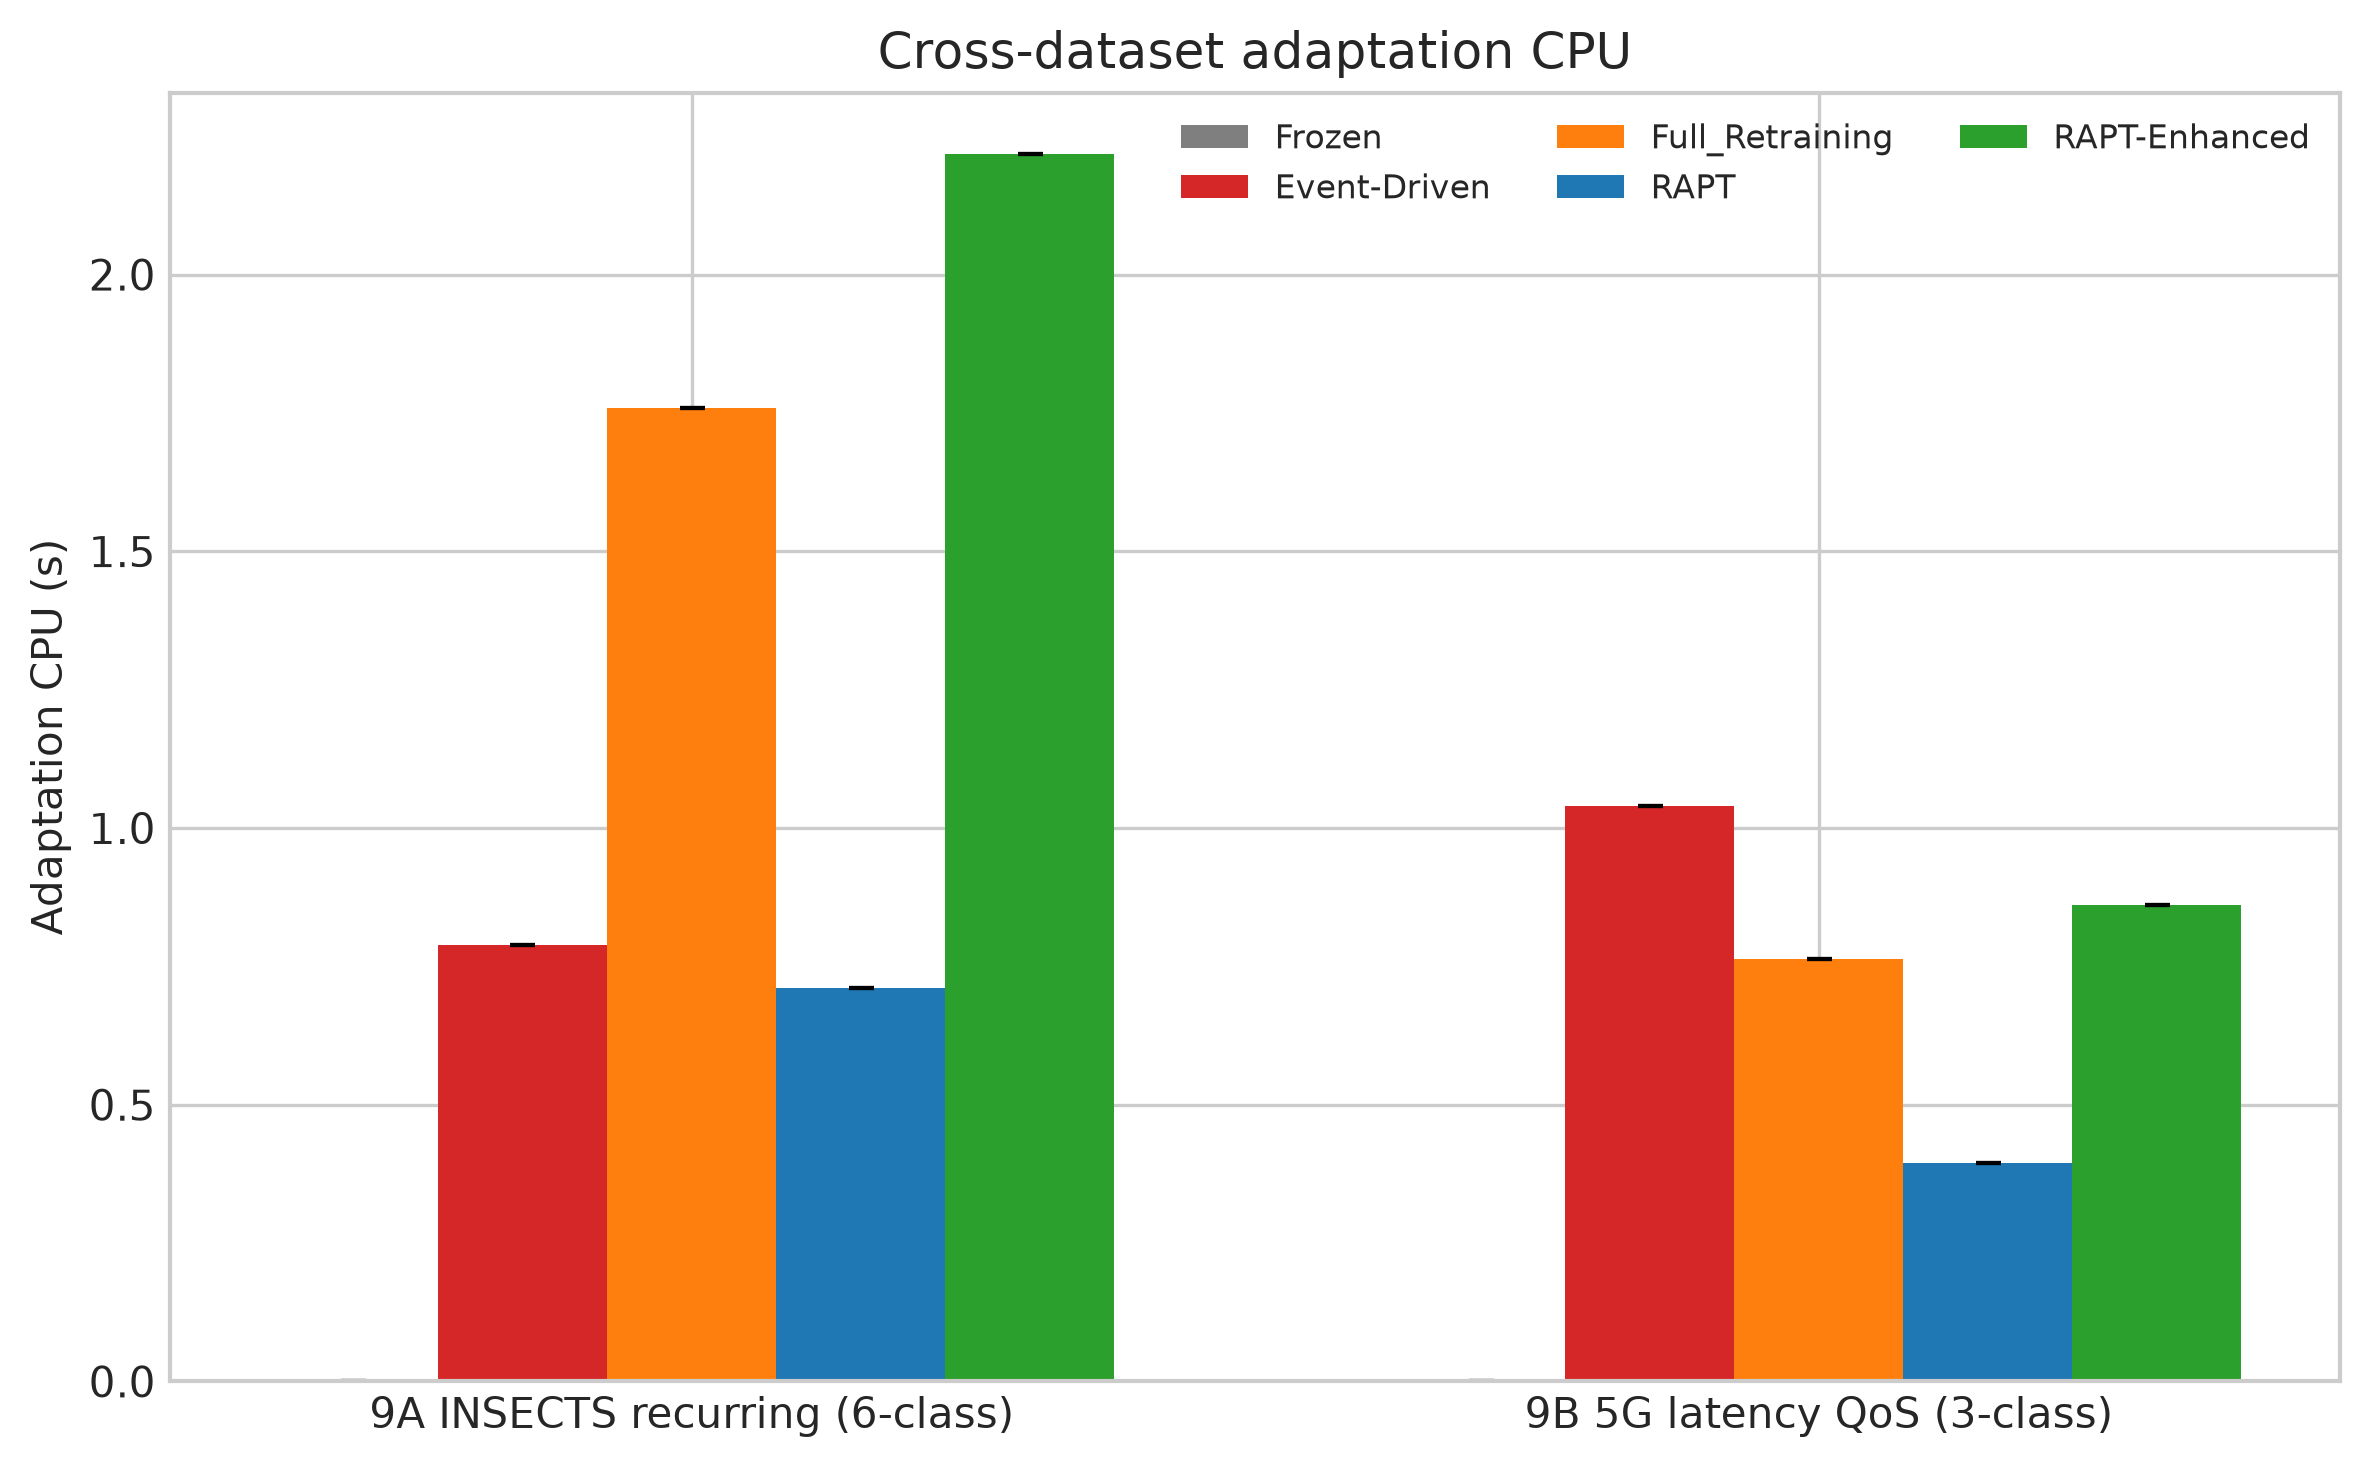
\includegraphics[width=\columnwidth]{computational_cost.png}
\caption{Adaptation CPU on the two largest streams. The ordering is the reverse of
Fig.~\ref{fig:primary}: on UGR'16, RAPT uses an order of magnitude less adaptation
time than Full Retraining and records lower macro-F1.}
\label{fig:cost}
\end{figure}


% ---------- NEW FIGURE: accuracy-cost trade-off across all four streams ----------
\begin{figure}[t]
\centering
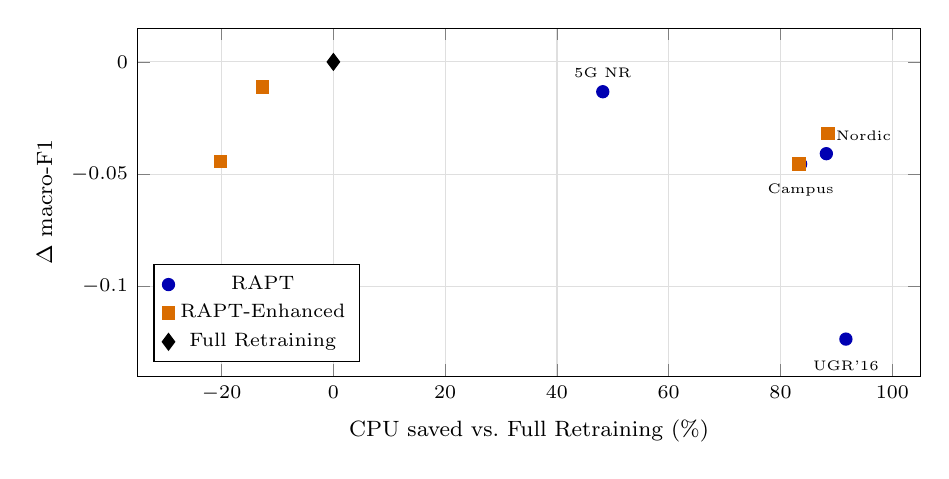
\begin{tikzpicture}
\begin{axis}[
  width=0.95\columnwidth, height=6cm,          % was width=\columnwidth, height=6.2cm
  xlabel={CPU saved vs.\ Full Retraining (\%)},% shorter
  ylabel={$\Delta$ macro-F1},                  % shorter, the caption already says "vs. Full Retraining"
  scaled y ticks=false,                        % kills the odd "5 · 10^-2" tick label
  yticklabel style={/pgf/number format/fixed, /pgf/number format/precision=2},
  xmin=-35, xmax=105, ymin=-0.14, ymax=0.015,
  grid=both, grid style={gray!25},
  tick label style={font=\scriptsize}, label style={font=\footnotesize},
  legend style={font=\scriptsize, at={(0.02,0.04)}, anchor=south west},
  every node near coord/.style={font=\tiny}]
\addplot[only marks, mark=*, mark size=2.2pt, blue!70!black] coordinates {
  (83.6,-0.0455) (91.7,-0.1235) (88.2,-0.0409) (48.2,-0.0133)};
\addplot[only marks, mark=square*, mark size=2.2pt, orange!85!black] coordinates {
  (83.3,-0.0455) (88.5,-0.0319) (-20.2,-0.0444) (-12.7,-0.0112)};
\addplot[only marks, mark=diamond*, mark size=3pt, black] coordinates {(0,0)};
\legend{RAPT, RAPT-Enhanced, Full Retraining}
\node[font=\tiny, anchor=north] at (axis cs:83.6,-0.050) {Campus};
\node[font=\tiny, anchor=north] at (axis cs:91.7,-0.129) {UGR'16};
\node[font=\tiny, anchor=south west] at (axis cs:88.2,-0.0395) {Nordic};
\node[font=\tiny, anchor=south] at (axis cs:48.2,-0.0115) {5G NR};
\end{axis}
\end{tikzpicture}
\caption{Accuracy--cost trade-off on all four streams, measured against Full
Retraining at the origin. Circles are RAPT and squares are RAPT-Enhanced, computed from
Table~\ref{tab:primary}. Up and to the right is better. Squares left of zero cost more
adaptation CPU than Full Retraining.}
\label{fig:scatter}
\end{figure}
% ---------- END NEW FIGURE ----------


\subsection{Efficiency Ablation}
\label{sec:ablation}
Table~\ref{tab:ablation} and Fig.~\ref{fig:ablation} show the mechanism ladder on 5G
Campus, in which each row adds one mechanism. RAPT-Full is the base controller with the
similarity gate, and it scores $0.9587 \pm 0.0000$ macro-F1 at $0.4283$\,s. Replacing the
absolute refit trigger with a relative-degradation trigger (RAPT-Evidence) leaves
macro-F1 unchanged and fires \emph{zero} refreshes. With an absolute floor (RAPT-Floor),
7.6 refreshes fire and the score is $0.9797 \pm 0.0050$ at $0.5865$\,s, higher than
before but noisier. RAPT-Cheap keeps the periodic schedule and uses the cheaper refit. Its score is
$0.9851 \pm 0.0029$ at $0.8477$\,s, compared with $0.9829 \pm 0.0023$ at $1.4063$\,s for
Full Retraining. The macro-F1 difference is $\Delta = +0.0022$ with $p = 0.3125$,
$d = 0.47$, and because the 95\% interval $[-0.0036, +0.0080]$ includes zero we cannot
claim a difference. The periodic refresh with a full refit scores $0.9847 \pm 0.0028$ at
$2.7168$\,s. Set against it, the cheap refit keeps the accuracy and cuts adaptation CPU
by roughly 69\%.
RAPT-Incremental scores $0.9549 \pm 0.0020$ at $0.5813$\,s. Against RAPT-Full
($0.9587$ at $0.4283$\,s) it is worse on both axes: lower macro-F1 and higher adaptation
CPU. It is therefore not carried forward. The mechanism that does survive is the periodic
schedule with the cheaper refit, RAPT-Cheap, which is the only configuration here that
combines accuracy on par with Full Retraining and a clear cost reduction.


\begin{table}[t] 
\caption{Performance of different configurations of RAPT using the 5G Campus stream, averaged over multiple random seeds.} 
\label{tab:ablation} 
\centering 
\footnotesize 
\begin{tabular}{@{}lccc@{}}
\toprule 
{\bf Configuration} & {\bf Macro-F1} & {\bf Adapt.\ CPU} & {\bf Refreshes}\\
\midrule 
Full Retrain. (ref.) & $0.9829 \pm 0.0023$& $1.4063$ & -- \\ 
RAPT-Full & $0.9587 \pm 0.0000$ & $0.4283$ & 0 \\ 
RAPT-Evidence & $0.9587 \pm 0.0000$ & $0.4260$ & 0\\ 
RAPT-Floor & $0.9797 \pm 0.0050$ & $0.5865$ & 7.6 \\ 
RAPT-Cheap & $\mathbf{0.9851 \pm 0.0029}$ & $0.8477$ & 22 \\ 
RAPT-Incremental & $0.9549 \pm 0.0020$ & $0.5813$ & 0\\ 
\bottomrule
\end{tabular}
\end{table}


\begin{figure}[t]
\centering
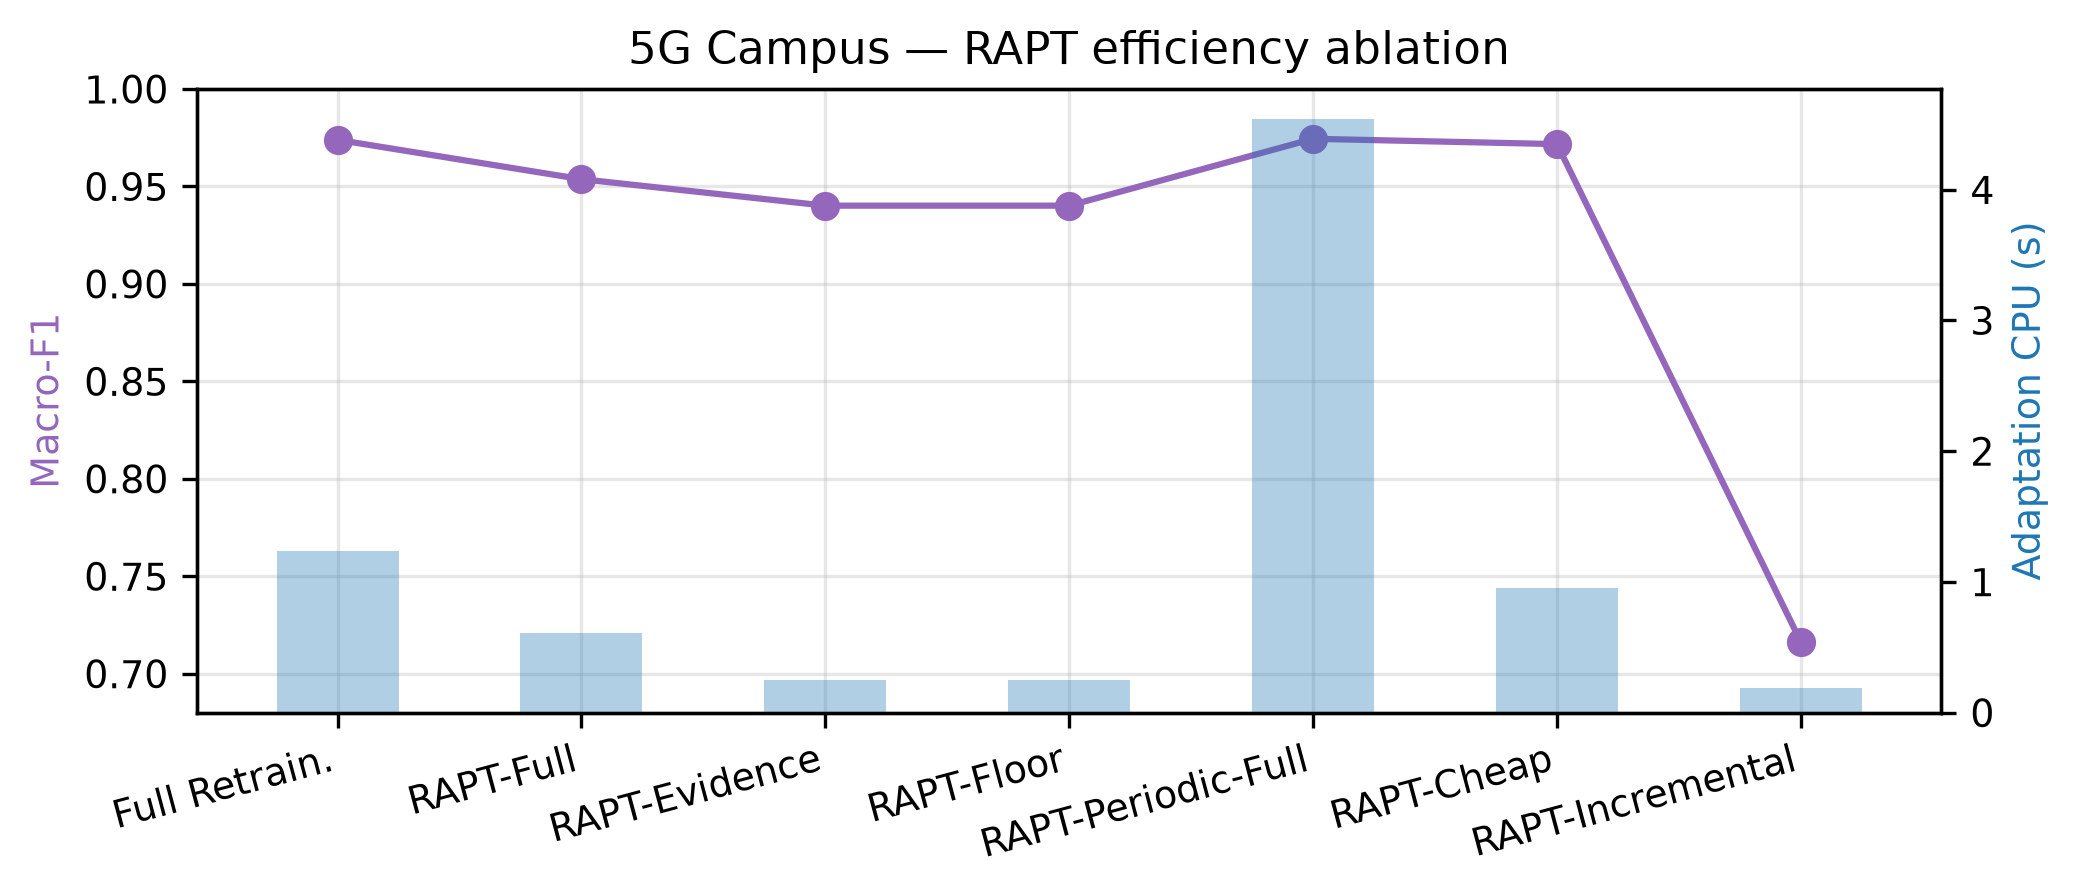
\includegraphics[width=\columnwidth]{rapt_ablation.png}
\caption{Ablation ladder comparing the different configurations of RAPT, evaluated on the 5G Campus stream. As shown, RAPT-Cheap matches the full retrainer in terms of macro-F1 at around $40\%$ less adaptation CPU, whereas RAPT-Incremental performs worse on both accuracy and cost. }
\label{fig:ablation}
\end{figure}


\subsection{Determinants of Cost and Trigger Behavior}
\label{sec:cost}
The cheap refresh was chosen from direct refit-timing measurements, varying one factor at a time with the ensemble held fixed: a 20-tree refit takes about 22\,ms against 104\,ms for 100 trees, and a 200-observation buffer about 80\,ms against 104\,ms for 1000 observations. Tree count dominates, so the cheap refit cuts refit time by about four-fifths at 20 trees.

\label{sec:trigger}
The zero-refresh result for RAPT-Evidence is a property of the mechanism, not a tuning
outcome. A relative trigger asks whether current accuracy has fallen by more than a margin
against a decayed reference built from that policy's own earlier accuracy. When a regime
is persistently poor rather than deteriorating, the reference decays toward the poor
level, the gap the rule tests for never opens, and the trigger stays silent even though
the policy is unfit. RAPT-Floor tests the same condition against a fixed floor and fires
7.6 refreshes where the relative rule fires none; that floor is stream-specific and would
need calibration elsewhere, which is why it is offered as a mechanism to be tuned rather
than a recommended constant.


\subsection{Comparison to Historical Detectors}
Of the four detectors, three never fire: ADWIN, Page-Hinkley and EDMA recorded zero
adaptation events on all three streams and so reproduce the frozen baseline by
construction. EDD fired 38--39 times per stream and reached the highest macro-F1 of any
method on 5G Campus ($0.9847 \pm 0.0019$) and NordicDat ($0.4184 \pm 0.0165$), at the
highest adaptation cost ($3.98$, $6.10$ and $4.69$\,s). RAPT fires 2--11 times per stream
depending on configuration. Its adaptation cost is below EDD's on all three datasets
($0.2292$ against $3.98$\,s on Campus, $1.9711$ against $6.10$\,s on UGR'16, $0.2594$
against $4.69$\,s on NordicDat), and on Campus its macro-F1 is within $0.002$ of EDD's.
On UGR'16 and NordicDat the cheaper trigger also yields lower macro-F1, so RAPT is the
lowest-cost adaptive option here rather than the most accurate one.



\begin{figure}[t]
\centering
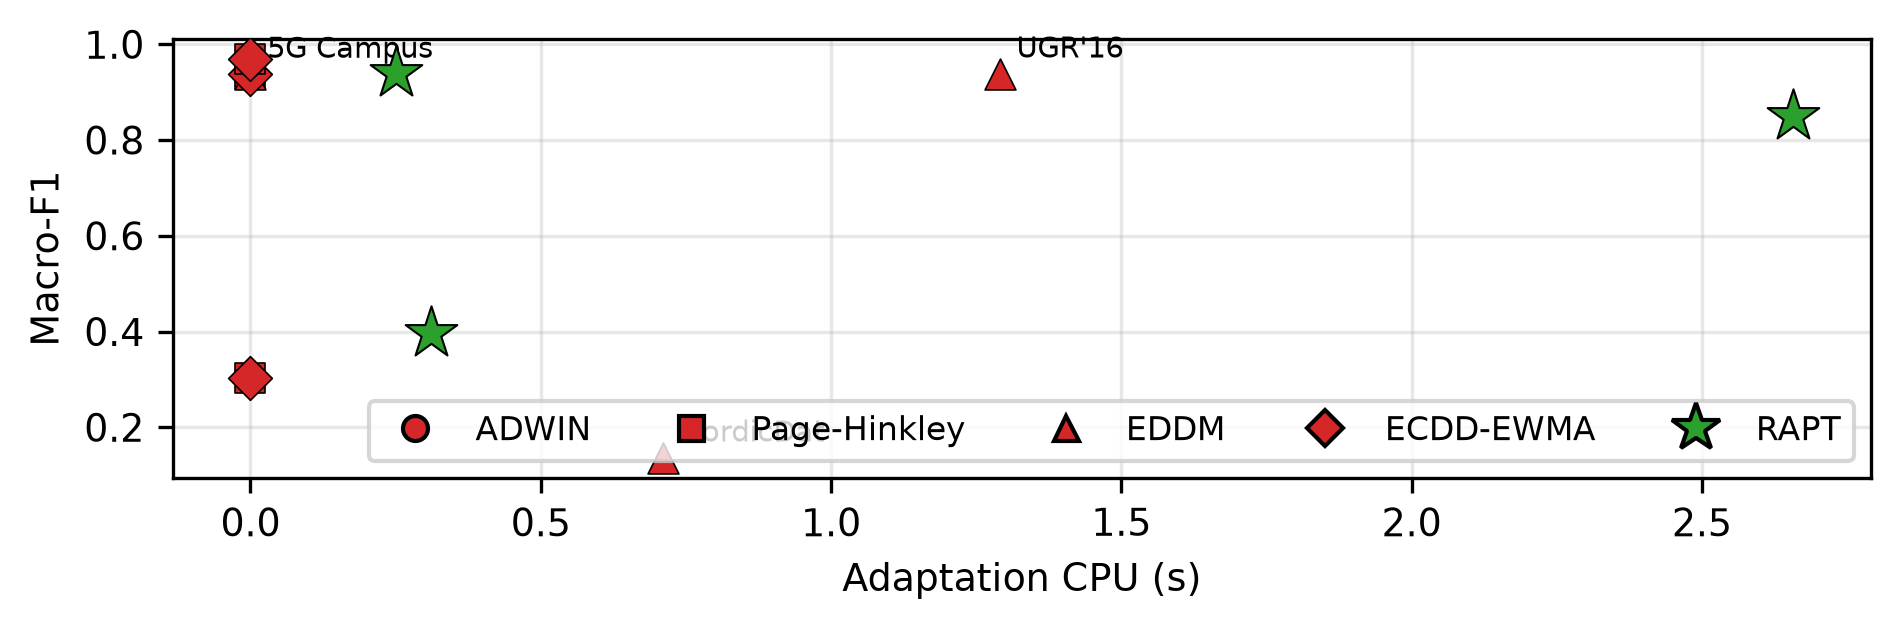
\includegraphics[width=\columnwidth]{detector_comparison.png}
\caption{Historical detectors comparison. Since ADWIN, Page-Hinkley and EDMA never fire they replicate the frozen baseline exactly. EDD fires most often and produces the highest macro-F1 at the highest adaptation cost. In contrast to these behaviors, RAPT has adapted less frequently than all but two of the methods studied here (and less accurately). } 
\label{fig:detector}
\end{figure}


\section{Discussion}


The mechanism is worth deploying when there is recurrence. The cost saving appears
wherever reuse occurs, but the accuracy penalty is concentrated on UGR'16, where regimes
recur and their label relationship does not. There a reused policy is stale, and the
parity refit earns its place by taking $0.8360$ to $0.9276$. For this reason reuse
should come with a check on the reused policy's recent performance. Reusing on the
regime identifier alone is unsafe when label semantics can drift independently of it.


\section{Independent Re-validation}
\label{sec:revalidation}

Every number here was re-derived from raw per-window records by a harness that
re-implements the streaming protocol rather than reading the committed aggregates. It
reproduces Tables~\ref{tab:primary} and~\ref{tab:ablation} to four decimal places on
every predictive metric, and an automated check of 199 quantitative claims against the
committed artifacts passes in full. Three findings are worth recording.

\emph{Cost is machine-dependent.} A re-run of the 9B drift pipeline reproduced every F1,
accuracy, precision and recall exactly but shifted adaptation CPU by up to $0.14$\,s. The
cost \emph{ordering} is stable and the gaps large (48--92\%); the absolute seconds are
indicative, not exact.

\emph{Retrieval keys do not track label semantics.} An oracle retraining on the previous
visit of the \emph{same} regime reaches only $0.5926 \pm 0.0077$ macro-F1 on UGR'16,
against $0.9595$ for Full Retraining, but $0.9905 \pm 0.0014$ on Campus. Regime identity
survives on Campus and not on UGR'16, exactly where blind reuse collapses. Recurrence
alone does not license reuse: on Campus a same-regime revisit predicts the previous visit
well (mean F1 $0.9876$), yet the class-conditional feature distributions differ by up to
a factor of $10^{8}$.

\emph{Controls.} On Campus a 20-tree cheap refit and a periodic 5-window schedule sit on
the cost--accuracy frontier and neither dominates RAPT-Cheap. A two-sided equivalence test
on UGR'16 rejects equivalence to Full Retraining at a $\pm0.005$ margin ($p = 0.95$), so
that gap is real and not a power artifact. A label-delay variant costs RAPT $0.13$
macro-F1 on NordicDat and $0.06$ on UGR'16 while leaving eager baselines unchanged; the
headline numbers assume labels arrive with their window.

\section{Limitations and Threats to Validity}
\label{sec:limitations}


Statistical power is the first concern. With five seeds, the smallest two-sided
$p$-value attainable in a seed-level comparison is $0.0625$, so some large effects
cannot reach formal significance, and this applies most to the ablation results.
Window-level tests assume that windows from one stream are independent, which inflates
the effective sample size and weakens any claim meant to generalise. Other limitations come from the design itself. The mechanism relies on regime
recurrence, which we measure and do not assume. A stream with no recurrence never
exercises the repository, and a novel regime falls back to retraining with no advantage
over the baseline. The RAPT-Floor threshold was calibrated on the evaluated stream, and
the 20-tree cheap refit was chosen for this particular ensemble. Both would have to be
revisited where the gap between pre- and post-drift data is larger, since a refit with
reduced capacity could underfit. The repository is never pruned, and the approach takes regime
similarity to be meaningful, which may fail if the regime signal is noisy.


\section{Conclusion}

Retraining is the standard response to drift, but when conditions return, part of what
was paid for is already in a previously trained model. RAPT keeps one policy per regime
and retrieves it on recurrence, training anew only when no suitable policy exists and
refreshing a stored policy once monitoring shows it no longer fits. Across four network
streams adaptation CPU was 48--92\% below full retraining, while macro-F1 was lower on
all four. Where regimes recurred with changed label relations, blind reuse caused
substantial damage; the parity-refit mechanism recovered most of it. Policy reuse is
worth deploying when regimes recur with consistent or monitored label meanings, and the
natural next step is to test whether a retrieved regime still means what it did when its
policy was stored.

\bibliographystyle{plain}
\bibliography{references}


\end{document}
